\documentclass[10pt,conference]{IEEEtran}
\usepackage{graphicx}
\usepackage{booktabs}
\usepackage{url}
\usepackage{cite}
\usepackage{amsmath}

\begin{document}

\title{Can Open-Source Multimodal LLMs Make Software-Engineering Figures Accessible?}

\author{
\IEEEauthorblockN{[FILL IN: Author Name(s)]}
\IEEEauthorblockA{[FILL IN: Affiliation]\\
Email: [FILL IN: email]}
}
% NOTE: SE4ALL 2027 uses SINGLE-BLIND review (confirmed via se4all.github.io,
% 2026-11-20) -- author names are NOT withheld, unlike double-blind venues.
% Fill in real author/affiliation details before submitting.

\maketitle

\begin{abstract}
Blind and low-vision (BLV) readers of software-engineering research papers have no reliable way to access the content of figures: captions are written for sighted readers and routinely assume the reader can already see what is being described. We study whether open-weight multimodal large language models (LLMs) are good enough, today, to generate accessible figure descriptions for SE papers -- a question with direct privacy and cost implications, since open models can be self-hosted rather than routed through a third-party API. We build a benchmark of 100 figures sampled from ICSE 2026 papers available on arXiv, stratified across charts, diagrams, and other common SE-paper figure types (qualitative examples, prompts, code screenshots), with 100 human-verified WCAG-style reference descriptions (full coverage of the evaluation sample). We evaluate four open-weight models and one closed baseline, each given \emph{only} the raw figure image, and score their output against the human reference on five accessibility-relevant criteria using an LLM-judge, spot-checked by the authors. Hallucination is pervasive across every model (55--86\% of descriptions contain at least one unsupported or contradicted claim), and -- counter to a naive open-vs-closed prior -- the closed baseline (GPT-4o, 60\%) is beaten by an open-weight model (Llama-4-Scout, 55\%); the largest open model evaluated (Gemma-3-27B) is also the worst (86\%). Charts are consistently harder than diagrams across models, consistent with the extra burden of precise numeric reading. We release the benchmark by reference (arXiv id + figure index + our descriptions + code, never the raw images) and discuss a roadmap toward accessible-by-default SE papers.
\end{abstract}

\section{Introduction}

Figures are not optional in software-engineering papers: architecture diagrams, pipelines, and empirical result charts routinely carry the paper's core claim. For a sighted reader, a figure plus its caption is usually enough. For a blind or low-vision (BLV) reader, the caption alone is frequently insufficient -- authors write captions assuming the reader can already see the figure (``as shown above,'' ``the red bars indicate...''), and in-text references to a figure (``Figure 3 shows that X outperforms Y'') presuppose the same. The result is that a large and growing body of SE research is effectively inaccessible to BLV researchers, reviewers, and practitioners, even though the venues publishing it increasingly frame accessibility as a first-class SE concern.

Large multimodal LLMs can, in principle, close this gap: given a figure, a vision-language model can generate a textual description a screen reader can read aloud. Closed, API-hosted models (GPT-4o, Gemini, Claude) are already capable of this in a general sense, but routing every figure a BLV researcher encounters through a third-party API is a real privacy and cost barrier -- an institution supporting BLV researchers at scale needs this to run locally, on infrastructure it controls. This motivates our central question: \textbf{are open-weight multimodal LLMs, used only on the figure image itself, good enough to generate accessible descriptions of SE-paper figures?}

We do not study ``how well do models read charts'' in the abstract -- that is a well-covered question (Section~\ref{sec:related}). Our contribution is specific to the SE-accessibility framing:
\begin{itemize}
\item A benchmark of 100 figures from ICSE 2026 papers on arXiv, stratified across chart, diagram, mixed, and other SE-paper figure types, released by reference with human-verified WCAG-style accessible reference descriptions;
\item An evaluation of four open-weight multimodal LLMs plus one closed baseline, given only the raw image (no caption, no surrounding text -- the realistic accessibility scenario), scored on five accessibility-relevant criteria by an LLM-judge against the human reference, with author spot-checks;
\item A hallucination-centric analysis: what specifically goes wrong when an open model misreads an SE figure, and whether that failure mode differs between statistical charts and SE diagrams;
\item A concrete roadmap for what it would take to make this reliable enough to deploy.
\end{itemize}

Given the venue and timeline, this is deliberately a lean, position-style study: we optimize for a defensible, honestly-reported result on a representative 100-figure sample rather than an exhaustive benchmark, and we say explicitly where we stopped and why.

\section{Related Work}
\label{sec:related}

\textbf{Scientific figure captioning and understanding.} SciCap~\cite{scicap} introduced a large-scale figure-caption dataset from arXiv papers (predominantly graph plots) and the task of generating a caption from a figure; SciCap+~\cite{scicapplus} extended this with additional context. Multimodal ArXiv / ArXivCap~\cite{arxivcap} scaled this further to 6.4M images across scientific domains and added captioning, QA, and title-generation tasks. SciFIBench~\cite{scifibench} instead poses figure understanding as a multiple-choice benchmark (figure-to-caption and caption-to-figure matching) and evaluates large multimodal models' interpretive, not just descriptive, capability. None of this prior work targets SE figures specifically, and none frames the task as accessibility: the ground truth in all three is a caption or caption-matching task, written for and evaluated against sighted-reader conventions.

\textbf{Accessible figure description.} Williams et al.~\cite{williams2022} analyzed alt text in published HCI papers and interviewed authors, finding that even domain experts struggle to write complete, accurate alt text for complex figures, and that existing captions are a poor substitute. FigurA11y~\cite{figura11y} built a human-AI collaborative tool (GPT-4 and LLaVA-assisted drafting with author revision) to help authors write better alt text, closest in spirit to our task but (a) assumes a human author in the loop at write-time, not a reader-side tool, and (b) evaluates on general scientific figures, not SE-specific charts and diagrams, and (c) uses closed models.

\textbf{Our positioning.} We combine the accessibility framing of Williams et al. and FigurA11y with the benchmark-construction rigor of SciCap/SciFIBench, applied to a domain (SE papers) neither line of work covers, and center the evaluation on open-weight, locally-deployable models -- a dimension prior accessibility tooling (built on closed APIs) does not address.

\section{Dataset Construction}

We build the benchmark from ICSE 2026 papers available on arXiv, released \emph{by reference} (arXiv id + figure index + our descriptions + code; never the raw images), which sidesteps copyright entirely regardless of each paper's license.

\textbf{Paper selection.} We extracted 322 paper titles from the ICSE 2026 proceedings table of contents and matched them against arXiv via the arXiv API (per-title query, not a full corpus scan -- with only $\sim$322 known titles, a targeted query is cheaper and faster than downloading and scanning the full arXiv metadata corpus). 195/322 titles (61\%) matched a paper on arXiv.

\textbf{Figure extraction.} For each matched paper we fetched the arXiv LaTeX source (PDF fallback when unavailable) and extracted each figure's image, author caption, and the in-text paragraphs that reference it (via \texttt{\textbackslash ref}-family macro mining), rasterizing vector graphics to PNG. Across 70 papers this yielded 639 candidate figures, of which 352 had a usable caption and image from clean LaTeX source (``good'' figures -- the rest came from rate-limited PDF fallback or papers without extractable captions and were not used further).

\textbf{Sampling and typing.} We tagged each good figure as \emph{chart}, \emph{diagram}, \emph{mixed}, or \emph{other} (qualitative examples, prompts, and code screenshots -- common in LLM4SE papers and not anticipated by a chart-vs-diagram framing, but kept as a distinct category rather than discarded) via a keyword heuristic over the caption and in-text mentions. We then drew a stratified random sample of 100 figures matching the natural type proportions of the 352-figure pool (38 chart, 23 diagram, 5 mixed, 34 other).

\textbf{Reference descriptions.} For each of the 100 figures we built a human-verified WCAG-style reference description (short alt text plus a 3--6 sentence long description covering figure type, structure, and key takeaway). To make this tractable, a strong model (Claude Sonnet) drafted each reference from the image plus the extracted caption/mentions (mirroring how a sighted author would read the paper to understand a figure), and 14 human annotators then reviewed every draft against the actual image. Flagged drafts were re-examined with the specific human critique and the image together, to distinguish genuine visual errors (corrected) from critiques asking for analytical content not actually depicted in the image (where describing only what is visible is correct behavior for this task, not a flaw, and the draft was kept). All 100 references were completed this way.

\section{Evaluation Protocol}

\textbf{Models.} We evaluate four open-weight multimodal LLMs spanning four labs (Qwen3-VL-8B, Llama-4-Scout, Gemma-3-27B, Mistral-Small-3.2-24B) plus one closed baseline (GPT-4o), all via hosted inference (API access, not locally deployed, due to evaluator hardware constraints -- see Limitations). GPT-4o serves only as a reference point for ``how far from frontier closed-model quality are we,'' not as a contribution of this paper.

\textbf{Task.} Each model receives \emph{only} the raw figure image and is asked to produce a WCAG-style accessible description (short alt text plus a 3--6 sentence long description), with no caption or surrounding text. This is deliberate: giving the model the caption would test paraphrasing, not vision, and would not match the realistic scenario a BLV reader faces when a caption is itself insufficient.

\textbf{Scoring.} An LLM-judge (Claude Sonnet, distinct from the closed baseline to reduce self-preference risk) scores each generated description against the human reference, grounded in the image itself, on five criteria: (1) \emph{factual accuracy} (1--5), (2) \emph{hallucination} (binary, with the specific false claim identified when present) -- our headline safety metric, (3) \emph{completeness} (1--5), (4) \emph{message conveyed} (1--5, does the description communicate why the figure matters, not just its literal contents), and (5) \emph{conciseness} (1--5). We deliberately do not lead with BLEU/ROUGE: surface text-overlap metrics penalize valid paraphrasing and do not detect hallucination, the failure mode this study centers on. Judge outputs were spot-checked by the authors against the source images.

\section{Results}
\label{sec:results}

We scored 492/500 model outputs (5 models $\times$ 100 figures, minus 8 judge calls that failed to parse after retries and were dropped rather than retried indefinitely). Table~\ref{tab:results} summarizes all five criteria per model.

\begin{table}[t]
\centering
\caption{Mean score per criterion (1--5) and hallucination rate (\%, lower is better) per model.}
\label{tab:results}
\footnotesize
\begin{tabular}{lccccc}
\toprule
Model & Acc. & Compl. & Msg. & Conc. & Halluc.\% \\
\midrule
Qwen3-VL-8B           & 3.0 & 2.6 & 3.0 & 4.1 & 71.4 \\
Llama-4-Scout         & 2.6 & 2.1 & 2.2 & 3.8 & \textbf{54.6} \\
Gemma-3-27B           & 2.5 & 2.3 & 2.6 & 3.8 & 85.7 \\
Mistral-Small-3.2-24B & 2.9 & 2.4 & 2.8 & 4.0 & 62.0 \\
GPT-4o (closed)       & \textbf{3.1} & \textbf{2.5} & 2.8 & \textbf{4.2} & 59.6 \\
\bottomrule
\end{tabular}
\end{table}

\textbf{Hallucination is the dominant failure mode, for every model, including the closed baseline.} Fig.~\ref{fig:halluc} shows the per-model hallucination rate: from 54.6\% (Llama-4-Scout) to 85.7\% (Gemma-3-27B). Strikingly, \textbf{GPT-4o is not the best performer} -- at 59.6\% it is beaten by an open-weight model (Llama-4-Scout, 54.6\%) and only narrowly ahead of Mistral-Small-3.2-24B (62.0\%). Openness, by itself, is not what separates the reliable models from the unreliable ones here.

\textbf{Scores on the four Likert criteria are consistently mediocre, not catastrophic} (Fig.~\ref{fig:scores}): accuracy ranges 2.50--3.06/5, completeness 2.08--2.64/5, message-conveyed 2.2--2.96/5, conciseness 3.77--4.22/5 (the easiest criterion for every model -- length control is not the problem). Gemma-3-27B is the weakest model on every criterion despite being the largest open model evaluated, underscoring that parameter count alone does not predict accessibility-description quality.

\begin{figure}[t]
\centering
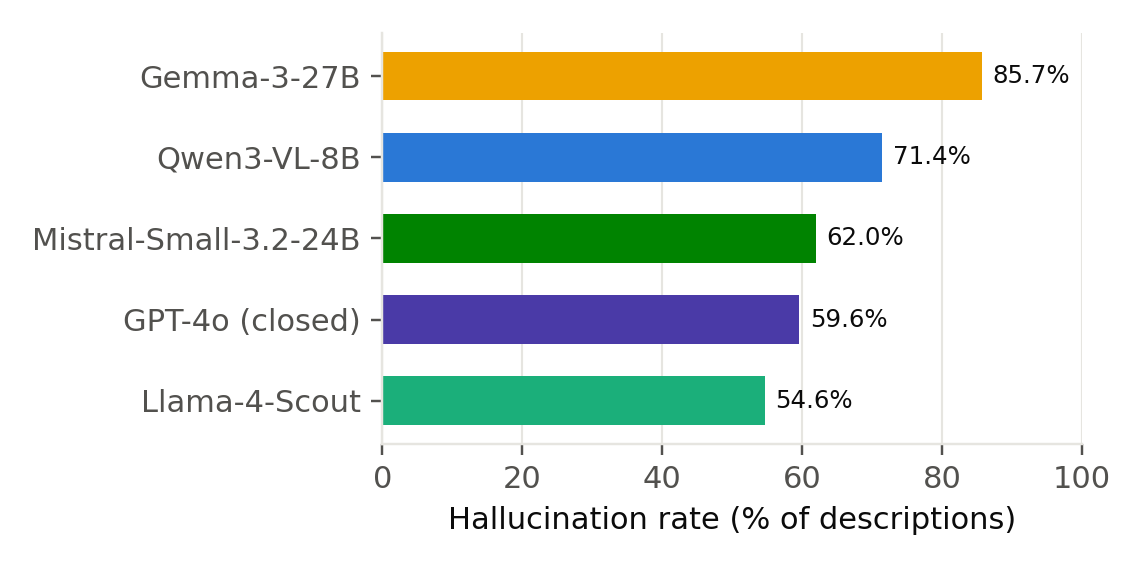
\includegraphics[width=\columnwidth]{figures/hallucination_rate.png}
\caption{Hallucination rate per model. The closed baseline (GPT-4o) is not the safest option; an open-weight model (Llama-4-Scout) hallucinates least.}
\label{fig:halluc}
\end{figure}

\begin{figure}[t]
\centering
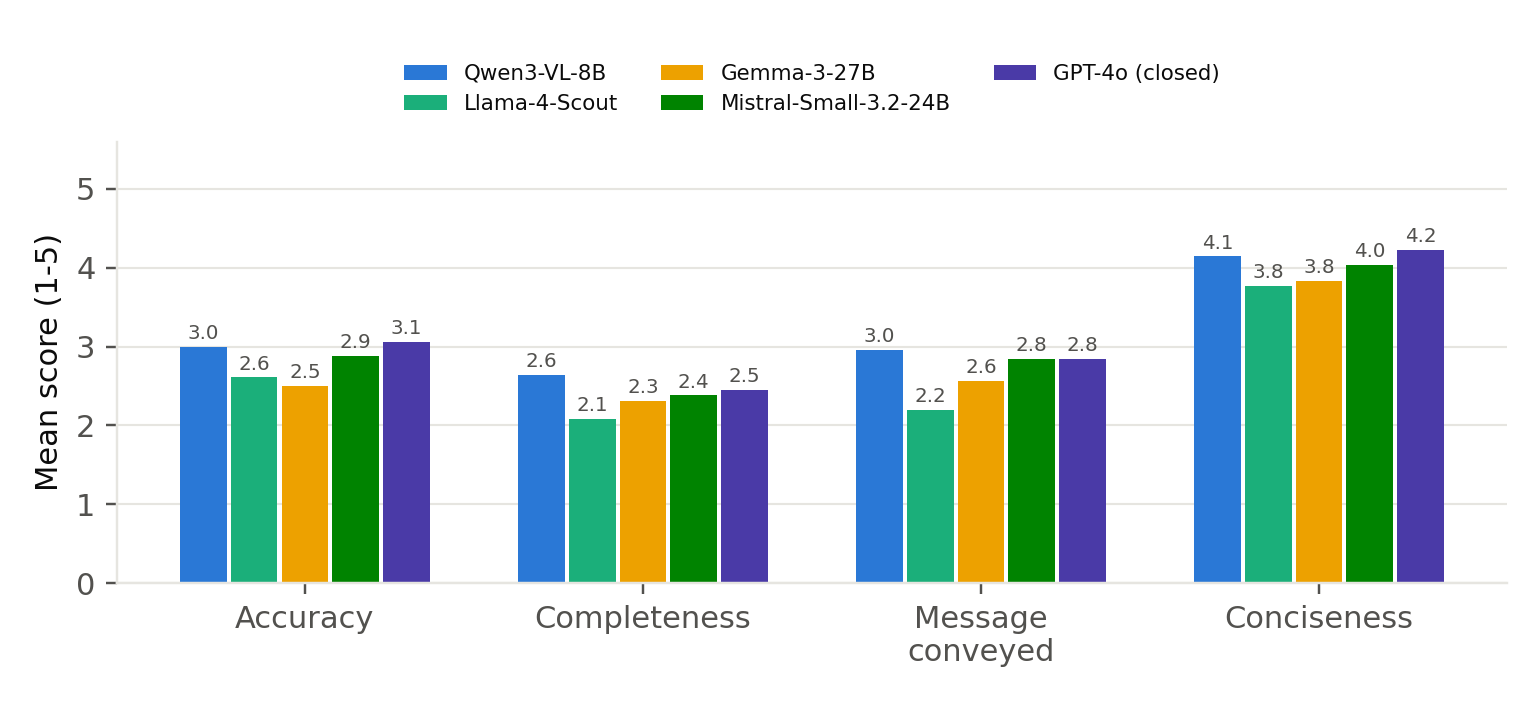
\includegraphics[width=\columnwidth]{figures/scores_by_criterion.png}
\caption{Mean judge score (1--5) per model across the four Likert criteria.}
\label{fig:scores}
\end{figure}

\textbf{Charts are harder than diagrams, for every model that shows a clear split.} Fig.~\ref{fig:erroranalysis}(a) breaks hallucination rate down by figure type. Four of five models hallucinate more on charts than on diagrams (Qwen3-VL-8B: 79\% vs.\ 69\%; Llama-4-Scout: 63\% vs.\ 39\%; Gemma-3-27B: 97\% vs.\ 76\%; GPT-4o: 74\% vs.\ 56\%); only Mistral-Small is roughly flat across types (61\% vs.\ 64\%). This is consistent with charts demanding precise numeric/trend reading (exact rankings, magnitudes, crossover points) where diagrams mostly require correctly tracing discrete structure and labeled relationships -- a plausibly easier visual task. The \emph{mixed} and \emph{other} categories have small counts (3 and 25 of 100 figures respectively) and should be read as indicative, not conclusive.

\begin{figure}[t]
\centering
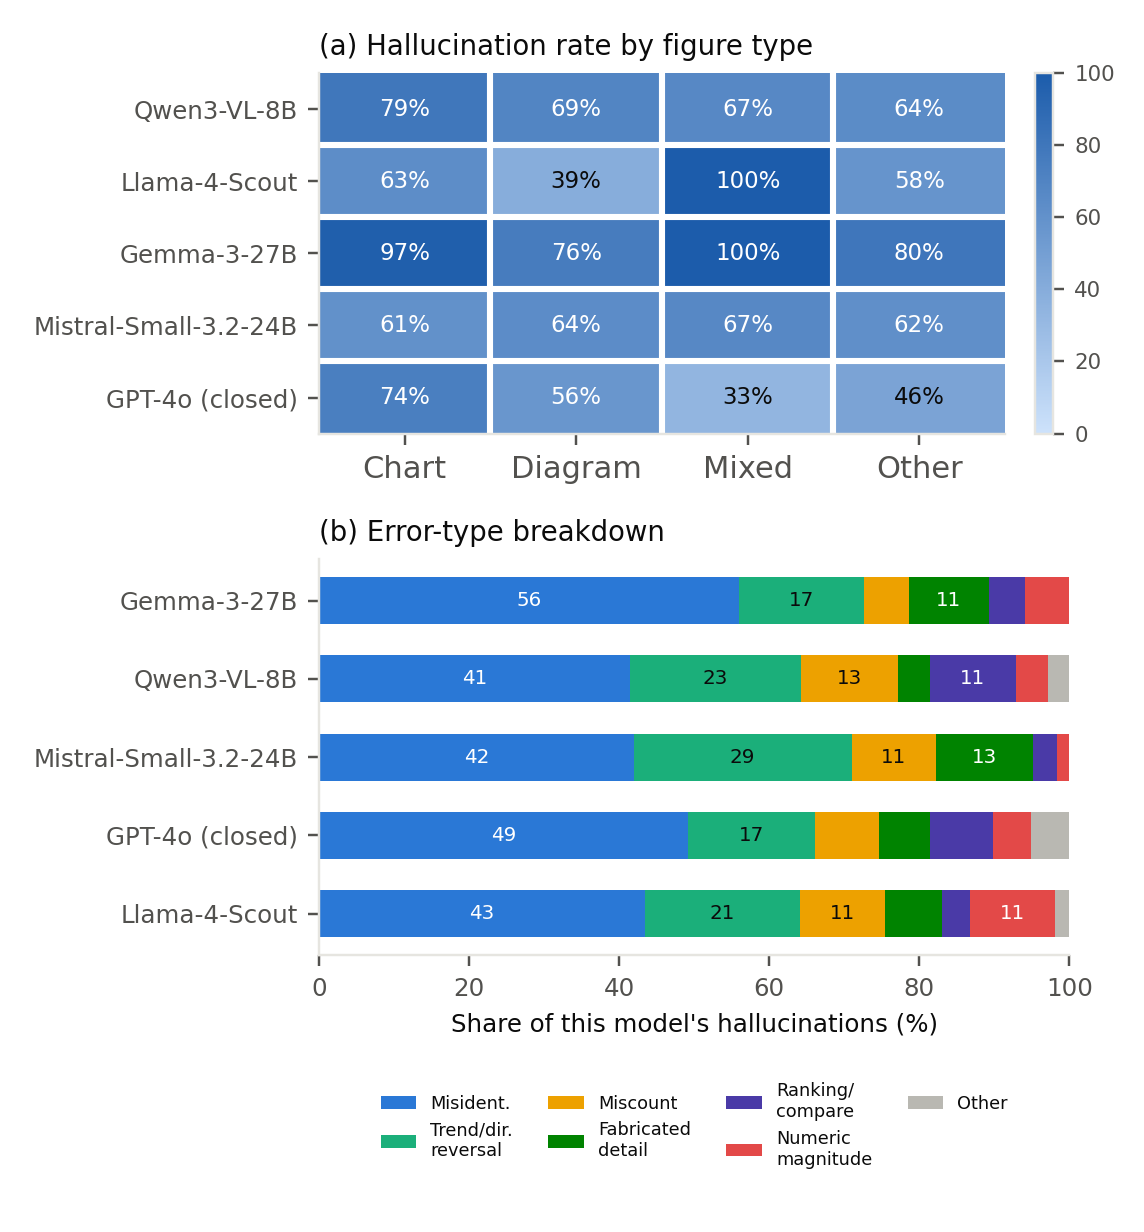
\includegraphics[width=\columnwidth]{figures/error_analysis.png}
\caption{(a) Hallucination rate by model and figure type. (b) Share of each model's hallucinations by error type (models sorted by total hallucination count).}
\label{fig:erroranalysis}
\end{figure}

\section{Discussion}

\textbf{A single figure, five different wrong rankings.} All five models hallucinated on the same chart (a two-panel box-plot comparison of code-agent pass rates, arXiv 2511.03153, fig.\ 11) -- and each invented a \emph{different} specific ranking error: Qwen3-VL-8B claimed GPT and StarCoder led when DeepSeek-Coder's median was actually highest; Llama-4-Scout made the same GPT-led claim; Gemma-3-27B reversed the entire directional trend (``context lowers pass rates'' when the figure shows the opposite); GPT-4o repeated the DeepSeek-Coder omission independently. No two models failed identically, which suggests these are not a shared training-data artifact but each model genuinely misreading the chart's visual structure (which box is tallest, which median line is highest) under its own vision encoder's limitations -- a harder problem to fix with better prompting alone.

\textbf{Why do some models hallucinate more than others?} To move past the aggregate rate, we classified all 328 hallucinated claims into six categories (one author-defined taxonomy, applied by the same LLM-judge given only the claim text): \emph{misidentification} (wrong label/identity of a visible element), \emph{trend/direction reversal}, \emph{miscount}, \emph{fabricated detail} (asserting something not depicted at all), \emph{ranking/comparison} error, and \emph{numeric magnitude} error. Fig.~\ref{fig:erroranalysis}(b) shows the per-model profile.

Three findings are worth stating precisely, with appropriate caution given the modest per-cell sample sizes (53--84 hallucinations per model, so individual category counts can be in the single digits):

\emph{(1) Misidentification is the dominant failure mode for every model (41--56\%), not a differentiator.} Every model's single largest error category is getting the identity of a visible element wrong (an icon, a legend entry, an axis label) rather than a higher-level reasoning failure. This suggests the primary bottleneck across the board is low-level visual grounding, not description composition -- consistent with the roadmap's emphasis on a grounding/verification pass rather than better prompting.

\emph{(2) Gemma-3-27B's weakness is concentrated, not uniform.} It has both the highest misidentification share (56\%, vs.\ 41--49\% for the others) and the highest fabricated-detail share (11\%, tied with Mistral-Small at 13\%). Combined with it being the largest \emph{dense} open model evaluated, this points to a specific weakness in visual grounding and calibration rather than a general capability deficit -- parameter count did not buy it more careful reading of the image.

\emph{(3) Llama-4-Scout's edge is calibration, not a cleaner profile.} Its error-type distribution (43\% misidentification, 21\% trend reversal, 11\% miscount, 8\% fabricated detail) is not dramatically different in \emph{shape} from the other models -- what differs is that it hallucinates less \emph{overall} (Table~\ref{tab:results}) while keeping its lowest-severity category (fabricated detail, arguably the most avoidable error -- there is nothing in the image to have gotten wrong) at the lowest rate of any model. A weak but directionally consistent signal in the same direction: mean description length correlates positively with hallucination at the individual-example level (Pearson $r=0.17$, $n=492$) -- Llama-4-Scout and GPT-4o, the two lowest-hallucination models, also write the shortest descriptions (93 and 96 words on average, vs.\ 112--114 for the other three). This is consistent with, though does not prove, a simple mechanism: more asserted claims is more surface area for an error, and the best-calibrated models may be implicitly hedging by saying less.

Trend/direction-reversal errors (17--29\%) are the most uniform category across models -- every model gets confused about whether a line goes up or down, or whether removing a condition raises or lowers a metric, at roughly similar rates. This is the category least explained by which model you pick, and the strongest argument for the grounding-based mitigation below rather than model selection alone.

\textbf{Roadmap.} Three directions follow directly from these results. First, \emph{chart-specific grounding}: since misidentification and trend-reversal errors dominate uniformly, a practical mitigation is a preprocessing step that extracts approximate numeric values and calibrates axes before generation, rather than asking the end-to-end model to both read and describe in one pass. Second, \emph{verification before delivery}: given hallucination rates this high, a BLV-facing accessibility tool cannot respond with a raw single-pass generation -- a second, cheaper verification pass (did every claim in the description appear in an OCR/structured read of the figure?) is close to necessary before the description reaches a reader who cannot independently check it. Third, \emph{benchmark-driven model selection}: since neither parameter count nor closed-vs-open status predicted performance here, a real deployment should select by measured error profile on a task-representative sample, not by defaulting to the largest or most prominent available model.

\textbf{On scaling this benchmark.} We evaluated and fully human-verified 100 of 352 extracted figures. The remaining 252 extracted figures (and any further ICSE/FSE/ASE papers not yet processed) are a natural next step: both for statistical power on the per-type breakdown (the mixed/other cells above have only 3 and 25 samples) and as a fine-tuning dataset -- but a fine-tuning target set needs human-verified descriptions, not raw model outputs, since fine-tuning on a model's own unverified generations would reinforce rather than correct the failure modes documented here.

\section{Limitations}

Our evaluation sample (100 of 352 extracted figures) is intentionally representative rather than exhaustive, consistent with this paper's position-paper framing; we report the full 352-figure extraction pipeline and plan to grow the human-verified reference set beyond this submission. Open-weight models were evaluated via hosted inference rather than literally run on local hardware, because the evaluation machine (8GB RAM) cannot host even a small vision-language model alongside the rest of the pipeline; we treat ``open-weight and therefore self-hostable by an adopting organization'' as the relevant claim, not ``we personally ran it locally.'' Our LLM-judge, while spot-checked, is itself a model and inherits the general risks of LLM-as-judge evaluation (surface-feature bias, inconsistency); we mitigate this with a structured, auditable rubric and rationale output rather than a single opaque score.

\section{Conclusion}

Open-weight multimodal LLMs are not yet reliable enough to generate accessible SE-figure descriptions unsupervised: every model we tested, including a leading closed baseline, hallucinated on more than half of the figures it described. But the headline finding for this venue is not ``not ready'' -- it is that \emph{open models are already competitive with, and in one case better than, a closed frontier model} on this task, which means the privacy and cost argument for local deployment does not require giving up quality today. The path forward is not a bigger model but a more careful pipeline around the model: chart-specific grounding, a verification pass before any description reaches a reader who cannot check it themselves, and benchmark-driven model selection over defaulting to scale. We release our 100-figure benchmark, protocol, and code to make that pipeline work measurable rather than assumed.

\bibliographystyle{IEEEtran}
\begin{thebibliography}{9}

\bibitem{scicap} T.-Y. Hsu, C. L. Giles, and T.-H. Huang, ``SciCap: Generating Captions for Scientific Figures,'' in \textit{Findings of the Association for Computational Linguistics: EMNLP 2021}, 2021.

\bibitem{scicapplus} Z. Yang, R. Dabre, H. Tanaka, and N. Okazaki, ``SciCap+: A Knowledge Augmented Dataset to Study the Challenges of Scientific Figure Captioning,'' \textit{arXiv:2306.03491}, 2023.

\bibitem{arxivcap} L. Li, Y. Wang, R. Xu, P. Wang, X. Feng, L. Kong, and Q. Liu, ``Multimodal ArXiv: A Dataset for Improving Scientific Comprehension of Large Vision-Language Models,'' in \textit{Proceedings of ACL 2024}, 2024.

\bibitem{scifibench} J. Roberts, K. Han, N. Houlsby, and S. Albanie, ``SciFIBench: Benchmarking Large Multimodal Models for Scientific Figure Interpretation,'' in \textit{NeurIPS 2024 Datasets and Benchmarks Track}, 2024.

\bibitem{williams2022} C. Williams, L. de Greef, E. Harris III, L. Findlater, A. Pavel, and C. Bennett, ``Toward Supporting Quality Alt Text in Computing Publications,'' in \textit{Proceedings of the 19th International Web for All Conference (W4A '22)}, Lyon, France, 2022.

\bibitem{figura11y} N. Singh, L. L. Wang, and J. Bragg, ``FigurA11y: AI Assistance for Writing Scientific Alt Text,'' in \textit{Proceedings of the 29th International Conference on Intelligent User Interfaces (IUI '24)}, 2024.

\end{thebibliography}

\end{document}
